\section{Software Design Konzepte}
Eine solide Softwarerchitektur ist entscheidend für die erfolgreiche Entwicklung und Wartung eines Programmes. Sie legt den Grundstein für die anschließende Implementierung. Durch eine gute Architektur wird sichergestellt das das Programm Skalierbar, Effizient, Robust und gut zu warten ist.\\
Hierbei bieten sogenannte Design Patterns abhilfe. \textit{Jedes Muster beschreibt zunächst ein in userer Umwelt immer wieder auftretendes Problem, beschreibt dann den Kern der Lösung dieses Problems, und zwar so dass man diese Lösung milionenfach anwendden kann, ohne sich je zu wiederholen} (Christof Alexander \textit{Eine Muster-Sprache} [Löcker verlag, Wien, 1995, Seite x]). Diese definition für muster bezieht sich auch auf objektorientierte Design Patterns. Das verwenden dieser Patterns ermöglicht Entwicklern von der Erfahrung anderer zu profitieren, um bereits gelöste Probleme nicht nochmal lösen zu Müssen. Zudem steigern sie auch die Codequalität. Der Code wird Lesbarer und die Wartung dessen wird leichter. Zudem wird auch die Implementierung neuer Erweiterungen und das Eindenken in die Software durch gängige Designpatterns erleichtert. \cite[S.25 ff]{DesignPatterns}\\
\textit{Alle gut strukturierten objektorientierten Architekturen basieren auf Mustern} (Grady Booch \cite[S.21]{DesignPatterns}).
In den folgenden Kapiteln wird genauer auf die in dieser Arbeit verwendeten Design Patterns eingegangen.      

\subsection{Adapter Pattern}
Zweck des Adapter Patterns ist die Anpassung der Schnitstelle einer Klasse an eine andere von dem Client erwarteten Schnitstelle. Somit ermöglicht das Pattern die Zusammenarbeit von zwei Klassen, welche auf grund ihrer Schnellen nicht möglich wäre. Das Adapter Patern ist auch unter dem namen Wrapper bekannt, welcher im folgenden Verlauf der arbeit verwendet wird.\\
Das Pattern kommt immer dann zum einsatz, wenn eine bereits existierende Klasse genutzt werden soll, jedoch die Schnitstelle der klasse nicht mit den aktuellen Anforderungen des clients übereinstimmt. Desweiteren wird das Dattern verwendet, wenn eine wiederverwendbare Klasse erzeugt werden soll, welche mit unabhängigen und nocht vorhersehbaren Klassen interagieren soll.\\      
\begin{center}
    \begin{figure}[h]
     \centering
     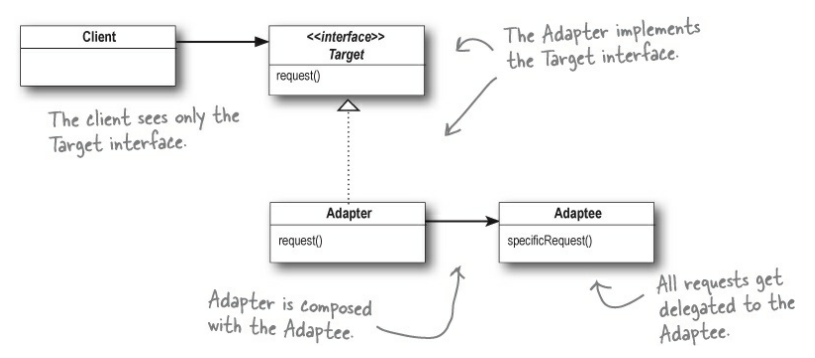
\includegraphics[width=1\linewidth]{UMLAdapterPattern}
     \caption{Adapter Pattern Struktur \cite{DesignPatterns}}
    \label{fig:AdapterPattern}
    \end{figure}
\end{center}
\vspace{-2cm}
Das Design Pattern besteht aus einem \textit{Target}, welches die vom Client verwendete Schnitstelle definiert. Zu dem kommt der \textit{Client}, welcher mit den Objekten zusammen arbeitet, die der Zielschnittstelle entsprechen. Zuletzt beinhaltet das Adapter Pattern einen \textit{Adaptee} so wie den \textit{Adapter} selbst. Der \textit{Adaptee} definiert eine bestehende Schnittstelle, welche vom \textit{Adapter} adaptiert werden muss.\\ 
Der \textit{Client} ruft die gewünschte Operation auf einer \textit{Adapter}-Instanz auf, welche anschließend die gewünschten \textit{Adaptee}-Operation ausführt.

\subsection{Strategie Design Pattern}
Zweck des Strategy (Strategie) Patterns ist es, eine Familie von einzelnen gekapselten und Austauschbaren Algorithmen zu schaffen. Dieses Patern ermöglicht eine variable und vom Client unabhöngige nutzung des Algorythmus.\\
Das Pattern kommt zum einsatz wenn eine Reihe von zusammenhängenden Klassen sich nur in Ihrem verhalten unterscheiden, verschiedene varianten eines Algorythmus erfordert werden, der Client keine Kenntnis von den vom Algorythmus verwendeten Daten haben soll, oder eine Klasse verschiedene Verhaltensweisen aufweist.\\
\begin{center}
    \begin{figure}[h]
     \centering
     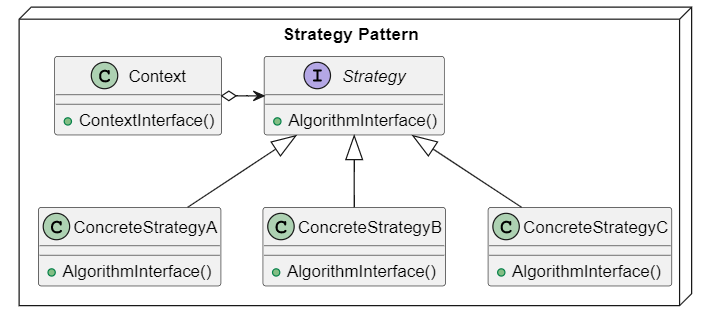
\includegraphics[width=1\linewidth]{UMLStrategyPattern}
     \caption{Strategie Pattern Struktur \cite{DesignPatterns}}
    \label{fig:StrategyPattern}
    \end{figure}
\end{center}
\vspace{-2cm}
Das Design Pattern besteht aus den folgenden Teilnehmern. Die \textit{Strategy}, welche eine gemeinsame Schnitstelle für die verwendeten Algorithmen deklariert. Einer oder mehreren \textit{ConcreteStrategy}, welche die Implementierung der Algorythmen oder Klassen ist, so wie dem \textit{Context}, welcher mit eier \textit{ConcreteStrategy} ausgestattet wird. Desweiteren bestitzt der \textit{Context} eine Referenz auf das \textit{Strategy} Objekt.\cite[S.383 ff]{DesignPatterns}\\
Über den \textit{Context} kann anschließend zur laufzeit des Programmes die benötigten \textit{ConcreteStrategy} geladen und ausgeführt werden. 
Ein konkretes Beispiel hierzu wird im buch \cite[Head First Design Patterns]{HeadfirstDesignPatterns} behandelt, was den nutzen dieses Patterns nochmal verdeutlicht.